\documentclass{beamer}

\usepackage{mathtools}
\usepackage{minted}
\usepackage{xcolor}
\usepackage[export]{adjustbox}
\usepackage{chemformula}

\usetheme{PaloAlto}
\usecolortheme{whale}

\setbeamertemplate{navigation symbols}{}

\title[MUSICA ODEs]{Overview of the \\
MUSICA
\footnote{Multi-Scale Infrastructure for Chemistry and Aerosols}
MICM
\footnote{Model-Independent Chemistry Module}
Library}

\author[Fillmore]{David Fillmore \\
\vspace{0.05in}
{\small \underline{ACOM
\footnote{Atmospheric Chemistry, Observations, and Modeling}
 MICM Group}}}

\vspace{-0.35in}

% \author[Fillmore]{David Fillmore\inst{NCAR,ACOM,M}}
% \institute[ACOM]{
% \inst{NCAR}%
% National Center for Atmospheric Research
% \and
% \inst{ACOM}%
% Atmospheric Chemistry, Observations, and Modeling Lab
% \and
% \inst{M}%
% Modeling Section
% }

\begin{document}

\frame{\titlepage}

\section{Chapman ODE Example}

\subsection{Chapman Mechanism}
\begin{frame}
\frametitle{Chapman Mechanism}
\vspace{-0.25in}
\begin{block}{Chapman Reactions}
\vspace{-0.2in}
\begin{align}
\mathrm{O_2} + \gamma &\rightarrow \mathrm{O}  + \mathrm{O} \tag*{molecular oxygen photolysis} \\
\mathrm{O} + \mathrm{O_2} + \mathrm{M} &\rightarrow \mathrm{O_3}  + \mathrm{M} \tag*{ozone creation} \\
\mathrm{O_3} + \gamma &\rightarrow \mathrm{O}  + \mathrm{O_2} \tag*{ozone photolysis (Chappuis)} \\
                      &\rightarrow \mathrm{O^*}  + \mathrm{O_2} \tag*{ozone photolysis (Hartley)} \\
\mathrm{O^*} + \mathrm{M} &\rightarrow \mathrm{O}  + \mathrm{M} \tag*{atomic oxygen quenching} \\
\mathrm{O} + \mathrm{O_3} &\rightarrow \mathrm{O_2}  + \mathrm{O_2} \tag*{ozone destruction}
\end{align}
\end{block}
% \vspace{-0.05in}
% {\it \small micm/examples/configs/chapman/reactions.json} \\
% \vspace{-0.15in}
\begin{block}{Chapman Species}
\begin{tabular}{|c|c||c|c|}
\hline
$\mathrm{O_2}$ & molecular oxygen
& $\mathrm{O}$ & atomic oxygen, ground state \\
$\mathrm{O_3}$ & ozone
& $\mathrm{O^*}$ & atomic oxygen, excited state \\
\hline
$\mathrm{M}$ & air molecule &
$\gamma$ & UV photon \\
\hline
\end{tabular}
\end{block}
\vspace{-0.05in}
% {\it \small micm/examples/configs/chapman/species.json}
{\small The Chappuis and Hartley branches are typically combined,
and $\mathrm{O^*}$ omitted from the mechanism.}

\end{frame}

\begin{frame}
\frametitle{Chapman ODEs}
\vspace{-0.25in}
\begin{block}{Chapman ODEs}
\vspace{-0.15in}
\begin{align*}
\frac{d}{dt} \left[ \mathrm{O} \right]
&=&
2 \ &j_2 \left[ \mathrm{O_2} \right]&
- &k_2 \left[ \mathrm{O} \right] \left[ \mathrm{O_2} \right]&
+ &j_3 \left[ \mathrm{O_3} \right]&
- &k_3 \left[ \mathrm{O} \right] \left[ \mathrm{O_3} \right]&
\\
\frac{d}{dt} \left[ \mathrm{O_2} \right]
&=&
- &j_2 \left[ \mathrm{O_2} \right]&
- &k_2 \left[ \mathrm{O} \right] \left[ \mathrm{O_2} \right]&
+ &j_3 \left[ \mathrm{O_3} \right]&
+ 2 \ &k_3 \left[ \mathrm{O} \right] \left[ \mathrm{O_3} \right]&
\\
\frac{d}{dt} \left[ \mathrm{O_3} \right]
&=&
& &
  &k_2 \left[ \mathrm{O} \right] \left[ \mathrm{O_2} \right]&
- &j_3 \left[ \mathrm{O_3} \right]&
- &k_3 \left[ \mathrm{O} \right] \left[ \mathrm{O_3} \right]&
\end{align*}
\end{block}
\vspace{0.05in}
\begin{tabular}{|c|c|c|c|}
\hline
$j_2$ & $k_2$ & $j_3$ & $k_3$ \\
\hline
$10^{-10}$ & $10^{-16}$ & $10^{-3}$ & $10^{-15}$ \\
s$^{-1}$ & cm$^3$ molecule$^{-1}$ s$^{-1}$
& s$^{-1}$ & cm$^3$ molecule$^{-1}$ s$^{-1}$ \\
\hline
\end{tabular}
\vspace{-0.05in}
\begin{exampleblock}{Dimensionless Concentrations
\hspace{0.2in} (both $j$ and $k$ units of s$^{-1}$)}
\vspace{0.05in}
$x_n = \left[ \mathrm{O}_n \right] /
\langle \left[ \mathrm{O_3} \right] \rangle
\hspace{0.1in} n = 1, 2, 3
\hspace{0.2in} \langle \left[ \mathrm{O_3} \right] \rangle
= 10^{12}$
molecules cm$^{-3}$ \\
$x_1 \sim 10^{-5} \hspace{0.2in}
x_2 \sim 2 \times 10^4 \hspace{0.2in} x_3 \sim 1$
\hspace{0.2in} $j_2 x_2 \sim 2 \times 10^{-6}$ s$^{-1}$
\\
$k_2 \sim 10^{-4}$ s$^{-1}$
\hspace{0.1in} $k_3 \sim 10^{-3}$ s$^{-1}$
\hspace{0.1in} $k_2 x_2 \sim 2$ s$^{-1}$
\end{exampleblock}

\end{frame}

\begin{frame}
\frametitle{3D and 2D Chapman Systems}
\vspace{-0.3in}
\begin{block}{3D Chapman System}
\vspace{-0.2in}
\begin{align*}
\frac{d}{dt}
\left( \begin{array}{c}
x_1 \\ x_2 \\ x_3
\end{array} \right)
=
\left( \begin{array}{ccc}
0 & 2 \ j_2 & j_3 \\
0 & - j_2 & j_3 \\
0 & 0 & - j_3 \\
\end{array} \right)
\left( \begin{array}{c}
x_1 \\ x_2 \\ x_3
\end{array} \right)
\\
+
k_2
\left( \begin{array}{c}
-1 \\ -1 \\ 1 
\end{array} \right)
x_1 x_2
+
k_3
\left( \begin{array}{c}
-1 \\ 2 \\ -1 
\end{array} \right)
x_1 x_3
\end{align*}
\end{block}
\vspace{-0.1in}
\begin{block}{2D Chapman System \ \ $x_2 = $ constant}
\vspace{-0.15in}
\begin{align*}
\frac{d}{dt}
\left( \begin{array}{c}
x_1 \\ x_3
\end{array} \right)
=
\left( \begin{array}{c}
2 \ j_2 x_2 \\ 0
\end{array} \right)
+
\left( \begin{array}{cc}
- k_2 x_2 & j_3 \\
k_2 x_2 & - j_3
\end{array} \right)
\left( \begin{array}{c}
x_1 \\ x_3
\end{array} \right)
\\
+ k_3
\left( \begin{array}{c}
-1 \\ -1
\end{array} \right)
x_1 x_3
\end{align*}
\end{block}
\vspace{-0.1in}
\begin{exampleblock}{}
\begin{equation*}
\frac{d}{dt} \left( x_1 + x_3 \right)
= 2 \ j_2 x_2 - 2 \ k_3 \ x_1 x_3
\end{equation*}
\end{exampleblock}

\end{frame}

\subsection{MICM Interface}
\begin{frame}
\begin{columns}
\begin{column}{0.47\textwidth}
\vspace{-0.25in}
\begin{block}{Molecular Oxygen Photolysis}
\begin{minted}{json}
{
  "type": "PHOTOLYSIS",
  "reactants": {
    "O2": {}
  },
  "products": {
    "O": {"yield": 2}
  },
  "MUSICA name":
    "molecular oxygen
     photolysis"
},
\end{minted}
\end{block}
\end{column}
\begin{column}{0.47\textwidth}
\vspace{-0.25in}
\begin{block}{Ozone Photolysis}
\begin{minted}{json}
{
  "type": "PHOTOLYSIS",
  "reactants": {
    "O3": {}
  },
  "products": {
    "O": {},
    "O2": {}
  },
  "MUSICA name":
    "ozone photolysis"
}]
\end{minted}
\end{block}
\end{column}
\end{columns}
\vspace{0.1in}
\small{Note photolysis rates typically vary with time and
are not specified in the configuration.}

\end{frame}

\begin{frame}
\begin{columns}
\begin{column}{0.47\textwidth}
\vspace{-0.33in}
\begin{block}{Ozone Creation}
\begin{minted}{json}
"name": "Chapman",
"type": "MECHANISM",
"reactions": [{
  "type": "ARRHENIUS",
  "reactants": {
    "O": {},
    "O2": {}
  },
  "products": {
    "O3": {}
  },
  "A": 1e-16,
  "MUSICA name":
    "ozone creation"
},
\end{minted}
\end{block}
\end{column}
\begin{column}{0.47\textwidth}
\vspace{0.04in}
\begin{block}{Ozone Destruction}
\begin{minted}{json}
{
  "type": "ARRHENIUS",
  "reactants": {
    "O": {},
    "O3": {}
  },
  "products": {
    "O2": {"yield": 2}
  },
  "A": 1e-15,
  "MUSICA name":
    "ozone destruction"
},
\end{minted}
\end{block}
\end{column}
\end{columns}

\end{frame}

\begin{frame}
\vspace{-0.27in}
\begin{block}{Python Interface}
\begin{minted}{python}
import musica

solver = musica.create_solver('configs/chapman',
    musica.micmsolver.rosenbrock, num_grid_cells)

n = 1e17 # molecules cm-3, lower stratosphere
# 0, 02, 03, rate ordering details omitted
concentrations = [1e-10 * n, 0.21 * n, 1e-5 * n]
rate_constants = {
    'PHOTO.molecular oxygen photolysis': 1e-10,
    'PHOTO.ozone photolysis': 1e-3}

musica.micm_solve(solver, time_step,
    temperature, pressure, air_density,
    concentrations, rate_constants)
\end{minted}
\end{block}

\end{frame}

\subsection{Phase Portraits}
\begin{frame}
\begin{columns}
\begin{column}{0.47\textwidth}
\vspace{-0.34in}
\begin{block}{Nonlinear Systems}
\begin{equation*}
\frac{d \mathbf{x}}{dt}
= \mathbf{F} \left( \mathbf{x}, t \right)
\end{equation*}
\begin{equation*}
\frac{dx_i}{dt}
= F_i \left( x_j, t \right)
\end{equation*}
% \begin{equation*}
% J_{ij} = \frac{\partial F_i}{\partial x_j}
% \end{equation*}
\end{block}
\vspace{-0.14in}
\end{column}
\begin{column}{0.47\textwidth}
\vspace{-0.34in}
\begin{block}{Linear Systems}
\begin{equation*}
\frac{d \mathbf{x}}{dt}
= \mathbf{s} \left( t \right) + L \left( t \right) \mathbf{x}
\end{equation*}
\begin{equation*}
\frac{dx_i}{dt}
= s_i \left( t \right) + \sum_{j=0}^N L_{ij} \left( t \right) x_j
\end{equation*}
\end{block}
\end{column}
\end{columns}
\vspace{-0.06in}
\begin{block}{Quadratic Systems}
\vspace{-0.2in}
\begin{equation*}
\frac{dx_i}{dt}
= s_i \left( t \right) + \sum_{j=0}^N L_{ij} \left( t \right) x_j
+ \frac{1}{2} \sum_{j=0}^N \sum_{k=0}^N Q_{ijk} \left( t \right) x_j x_k,
\ \ Q_{ikj} = Q_{ijk}
\end{equation*}
\end{block}
% \begin{block}{
% Power Series Expansion of $\mathbf{F} \left( \mathbf{x} + \mathbf{h} \right)$}
% \vspace{-0.22in}
% \begin{align*}
% F_i \left( x_j + h_j \right) = F_i \left( x_j \right)
% + \sum_{j=0}^N \frac{\partial F_i}{\partial x_j} h_j
% + \frac{1}{2} \sum_{j=0}^N \sum_{k=0}^N
% \frac{\partial F_i}{\partial x_j \partial x_k} h_j h_k
% + \cdots
% \end{align*}
% \end{block}
\vspace{-0.08in}
\begin{exampleblock}{Phase Space
[{\it Nonlinear Dynamics and Chaos}, Strogatz (2024)]}
\begin{itemize}
\item $\mathbf{x}$ a point in state space $\mathcal{M}, \dim{\mathcal{M} = N} $.
\item $\mathbf{F} \left( \mathbf{x}, t \right)$
a (time-dependent) vector field on $\mathcal{M}$.
\item $\mathbf{x} \left( \mathbf{x}_0, t \right)$
trajectories with initial conditions
$\mathbf{x} \left( \mathbf{x}_0, t_0 \right) = \mathbf{x}_0$.
\end{itemize}
\end{exampleblock}

\end{frame}

\begin{frame}
\begin{columns}
\begin{column}{0.65\textwidth}
\vspace{-0.35in}
\begin{figure}
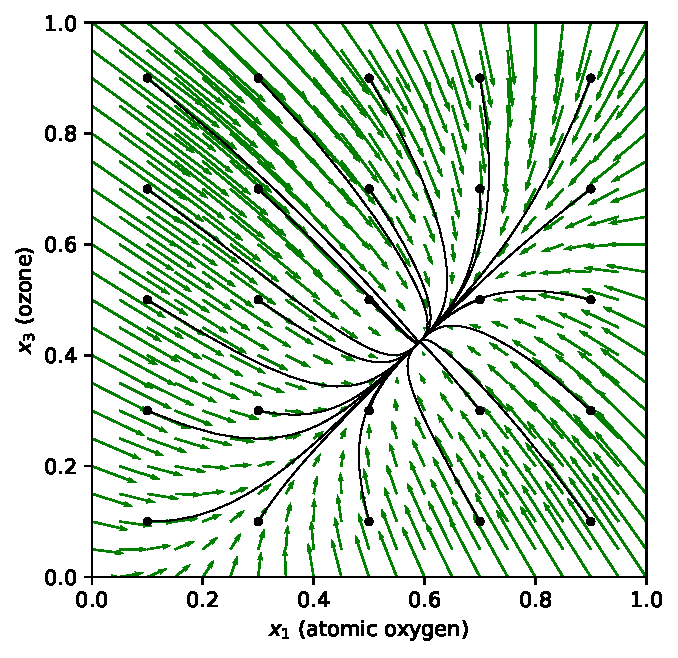
\includegraphics[scale=0.65]{../plots/chapman.pdf}
\end{figure}
\end{column}
\begin{column}{0.35\textwidth}
\vspace{-0.35in}
\begin{align*}
2 \ j_2 x_2 &= 0.1 \\
k_2 x_2 &= 0.3 \\
j_3 &= 0.3 \\
k_3 &= 0.2 \\
\end{align*}
\hspace{0.4in} $F_i$ scale $\frac{1}{2}$
\end{column}
\end{columns}

\end{frame}

\begin{frame}
\begin{columns}
\begin{column}{0.65\textwidth}
\vspace{-0.35in}
\begin{figure}
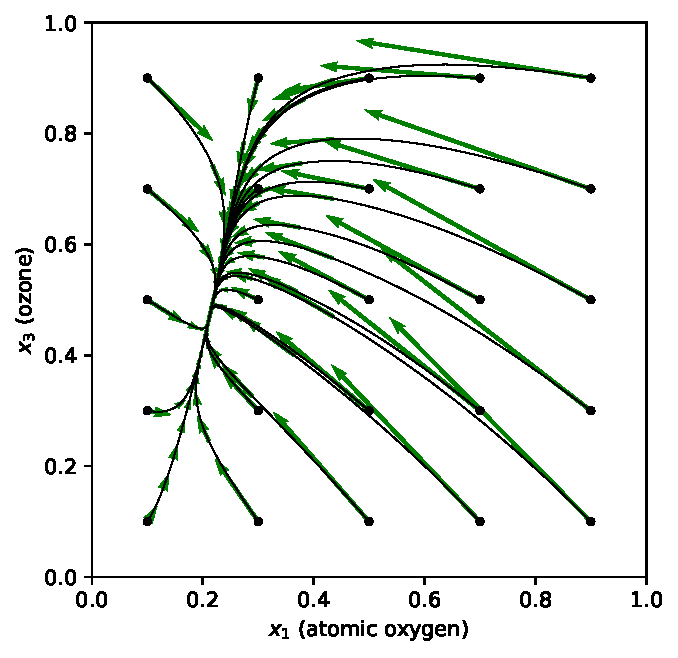
\includegraphics[scale=0.65]{../plots/chapman_1935.pdf}
\end{figure}
\end{column}
\begin{column}{0.35\textwidth}
\vspace{-0.35in}
\begin{align*}
2 \ j_2 x_2 &= 0.1 \\
k_2 x_2 &= 0.9 \\
j_3 &= 0.3 \\
k_3 &= 0.5 \\
\end{align*}
\hspace{0.4in} $F_i$ scale $\frac{1}{2}$
\end{column}
\end{columns}

\end{frame}

\begin{frame}
\begin{columns}
\begin{column}{0.65\textwidth}
\vspace{-0.35in}
\begin{figure}
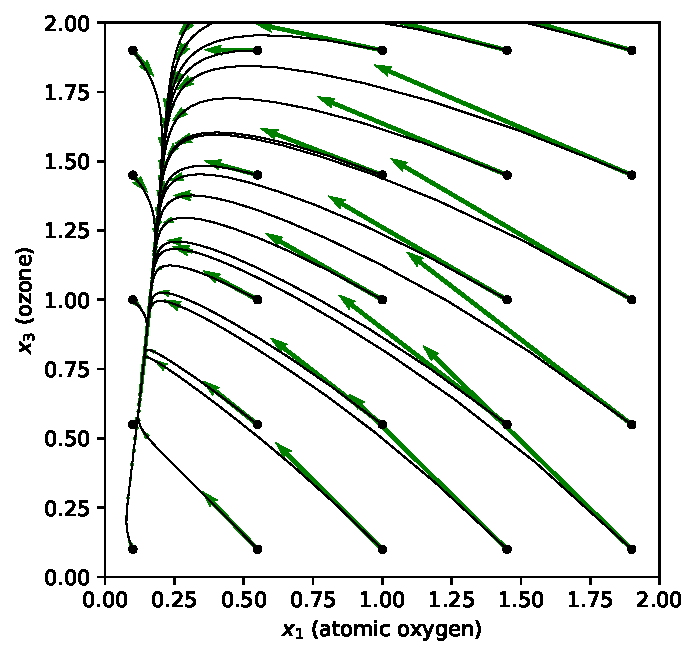
\includegraphics[scale=0.65]{../plots/chapman_fast.pdf}
\end{figure}
\end{column}
\begin{column}{0.35\textwidth}
\vspace{-0.35in}
\begin{align*}
2 \ j_2 x_2 &= 0.1 \\
k_2 x_2 &= 2.0 \\
j_3 &= 0.3 \\
k_3 &= 0.5 \\
\end{align*}
\hspace{0.4in} $F_i$ scale $\frac{1}{5}$
\end{column}
\end{columns}

\end{frame}

\section{Carbonic Acid DAE Example}

\subsection{Aqueous Chemistry}

\begin{frame}
\frametitle{Equilibrium Reactions}
\vspace{-0.2in}
\begin{block}{Henry's Law}
\begin{align*}
\ch{CO2(g) &<=> CO2(aq)} \quad &K_H &= \frac{[\ch{CO2(aq)}]}{P_{\ch{CO2}}}
\end{align*}
\end{block}

\begin{block}{Aqueous Equilibria}
\begin{align*}
\ch{H2O &<=> H+ + OH-} \quad &K_w &= [\ch{H+}][\ch{OH-}] \\[0.3cm]
\ch{CO2(aq) + H2O &<=> H+ + HCO3-} \quad &K_1 &= \frac{[\ch{H+}][\ch{HCO3-}]}{[\ch{CO2(aq)}]} \\[0.3cm]
\ch{HCO3- &<=> H+ + CO3^2-} \quad &K_2 &= \frac{[\ch{H+}][\ch{CO3^2-}]}{[\ch{HCO3-}]}
\end{align*}
\end{block}

\end{frame}

\begin{frame}
\frametitle{Charge Balance}

\begin{block}{Electroneutrality Constraint}
\begin{align*}
[\ch{H+}] &= [\ch{OH-}] + [\ch{HCO3-}] + 2[\ch{CO3^2-}] \\[0.3cm]
[\ch{H+}] &= \frac{K_w}{[\ch{H+}]} + \frac{K_1 K_H P_{\ch{CO2}}}{[\ch{H+}]} + \frac{2 K_1 K_2 K_H P_{\ch{CO2}}}{[\ch{H+}]^2}
\end{align*}
\end{block}

\begin{block}{pH Definition}
\begin{equation*}
\text{pH} = -\log_{10}[\ch{H+}]
\end{equation*}
\end{block}
\end{frame}

\begin{frame}
\frametitle{Equilibrium Constants}
\vspace{-0.22in}
\begin{table}
\centering
\begin{tabular}{|l|c|c|}
\hline
\textbf{Constant} & \textbf{Expression} & \textbf{Value} \\
\hline
$K_H$ & & $3.4 \times 10^{-2}$ M/atm \\[0.2cm]
$K_w$ & $k_{w}^{(f)} / k_{w}^{(r)}$ & $1.0 \times 10^{-14}$ M$^2$ \\[0.2cm]
$K_1$ & $k_{1}^{(f)} / k_{1}^{(r)}$ & $4.3 \times 10^{-7}$ M \\[0.2cm]
$K_2$ & $k_{2}^{(f)} / k_{2}^{(r)}$ & $4.7 \times 10^{-11}$ M \\
\hline
\end{tabular}
\end{table}
\begin{table}
\centering
\begin{tabular}{|l|c|}
\hline
\multicolumn{2}{|c|}{\textbf{Typical Results (400 ppm CO$_2$)}} \\
\hline
\textbf{Species} & \textbf{Concentration (M)} \\
\hline
pH & 5.65 \\
$[\ch{H+}]$ & $2.2 \times 10^{-6}$ \\
$[\ch{OH-}]$ & $4.5 \times 10^{-9}$ \\
$[\ch{CO2(aq)}]$ & $1.4 \times 10^{-5}$ \\
$[\ch{HCO3-}]$ & $2.7 \times 10^{-6}$ \\
$[\ch{CO3^2-}]$ & $5.8 \times 10^{-12}$ \\
\hline
\end{tabular}
\end{table}

\end{frame}

\begin{frame}
\begin{figure}
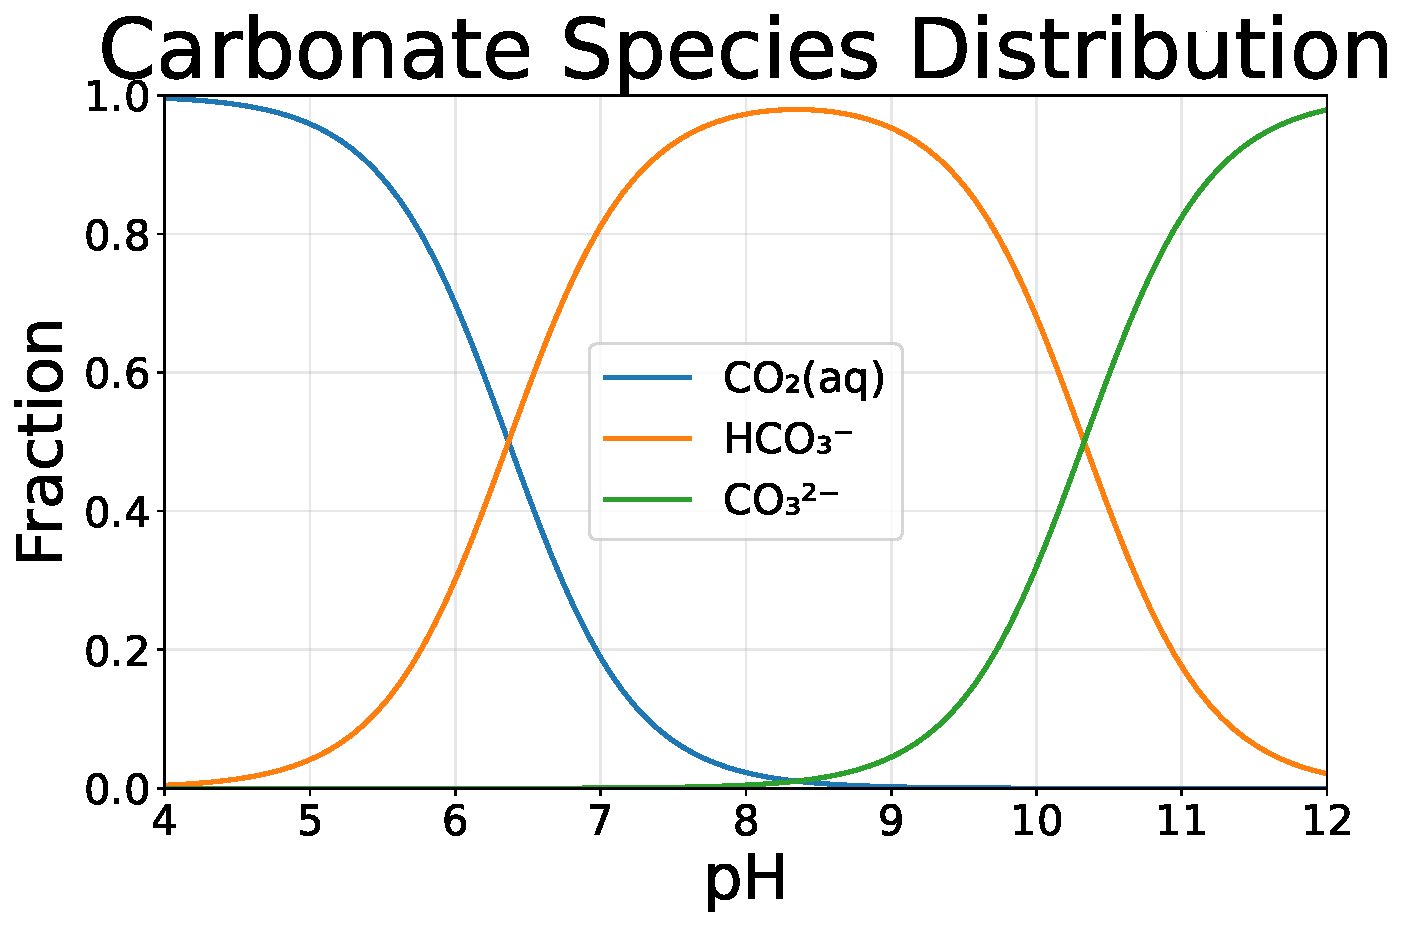
\includegraphics[scale=0.4]{../plots/carbonate_speciation.pdf}
\end{figure}
\end{frame}

\begin{frame}
\begin{figure}
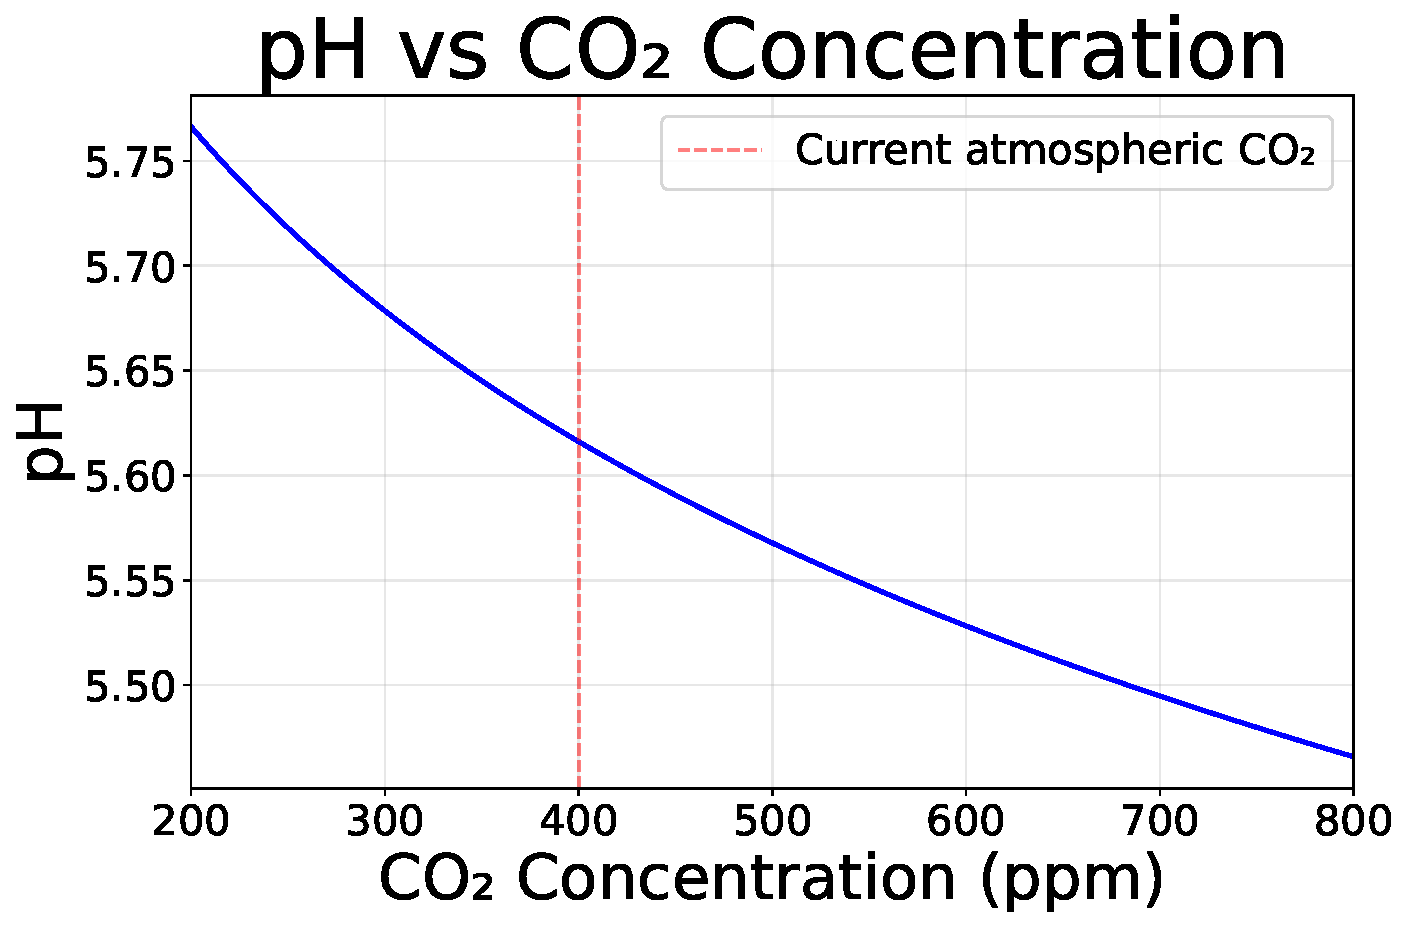
\includegraphics[scale=0.4]{../plots/pH_vs_CO2_concentration.pdf}
\end{figure}
\end{frame}

\section{Differential Algebraic Equations}
\frametitle{DAE System}

\begin{frame}
\begin{block}{Variable Definitions}
\begin{align*}
x_0 &= \frac{[\ch{CO2(aq)}]}{[\ch{CO2(aq, eq)}]} \\[0.3cm]
x_1 &= \frac{[\ch{HCO3^-}]}{[\ch{HCO3^-(eq)}]} \\[0.3cm]
x_2 &= \frac{[\ch{CO3^{2-}}]}{[\ch{CO3^{2-}(eq)}]} \\[0.3cm]
y &= \frac{[\ch{H^+}]}{[\ch{H^+(eq)}]}
\end{align*}
\end{block}

\end{frame}

\begin{frame}
\vspace{-0.2in}

\begin{block}{DAE System}
\begin{align*}
\frac{dx_0}{dt} &= \frac{1}{\tau_0}[1 - x_0] \\
\frac{dx_1}{dt} &= \frac{1}{\tau_1}[x_0 - x_1 \, y(x_1, x_2)] \\
\frac{dx_2}{dt} &= \frac{1}{\tau_2}[x_1 - x_2 \, y(x_1, x_2)] \\
y(x_1, x_2) &= \frac{A}{y(x_1, x_2)} + B_1 x_1 + B_2 x_2
\end{align*}
\end{block}

\begin{block}{Analytic Solution for $x_0$}
\begin{equation*}
x_0(t) = 1 + [x_0(0) - 1]e^{-t/\tau_0}
\end{equation*}
\end{block}

\end{frame}

\begin{frame}
\begin{block}{Discretized System}
\begin{align*}
F_0 &= x_0^{n+1} - x_0^n - \frac{\Delta t}{\tau_0}[1 - x_0^{n+1}] = 0 \\[0.2cm]
F_1 &= x_1^{n+1} - x_1^n - \frac{\Delta t}{\tau_1}[x_0^{n+1} - x_1^{n+1} y^{n+1}] = 0 \\[0.2cm]
F_2 &= x_2^{n+1} - x_2^n - \frac{\Delta t}{\tau_2}[x_1^{n+1} - x_2^{n+1} y^{n+1}] = 0 \\[0.2cm]
F &= \frac{A}{y^{n+1}} + B_1 x_1^{n+1} + B_2 x_2^{n+1} - y^{n+1} = 0
\end{align*}
\end{block}

\end{frame}

\begin{frame}
\vspace{-0.15in}
\begin{block}{$\partial \mathbf{F} / \partial \mathbf{x}$}
\begin{equation*}
\frac{\partial \mathbf{F}}{\partial \mathbf{x}} = \begin{bmatrix}
1 + \frac{\Delta t}{\tau_0} & 0 & 0 \\[0.3cm]
-\frac{\Delta t}{\tau_1} & 1 + \frac{\Delta t}{\tau_1} y & 0 \\[0.3cm]
0 & -\frac{\Delta t}{\tau_2} & 1 + \frac{\Delta t}{\tau_2} y
\end{bmatrix}
\end{equation*}
\end{block}

\vspace{-0.45in}
\begin{block}{$\partial \mathbf{F} / \partial y$}
\begin{equation*}
\frac{\partial \mathbf{F}}{\partial y} = \begin{bmatrix}
0 \\[0.3cm]
\frac{\Delta t}{\tau_1} x_1 \\[0.3cm]
\frac{\Delta t}{\tau_2} x_2
\end{bmatrix}
\end{equation*}
\end{block}

\end{frame}

\begin{frame}
\vspace{-0.1in}
\begin{block}{$\partial y / \partial \mathbf{x}$}
\begin{equation*}
\frac{\partial y}{\partial \mathbf{x}} = \frac{y^2}{A + y^2} \begin{bmatrix} 0 & B_1 & B_2 \end{bmatrix}
\end{equation*}
\end{block}

\vspace{-0.3in}
\begin{block}{Total Jacobian}
\begin{equation*}
\mathbf{J} = \frac{\partial \mathbf{F}}{\partial \mathbf{x}} + \frac{\partial \mathbf{F}}{\partial y} \frac{\partial y}{\partial \mathbf{x}}
\end{equation*}
\end{block}

\end{frame}

\begin{frame}
\begin{figure}
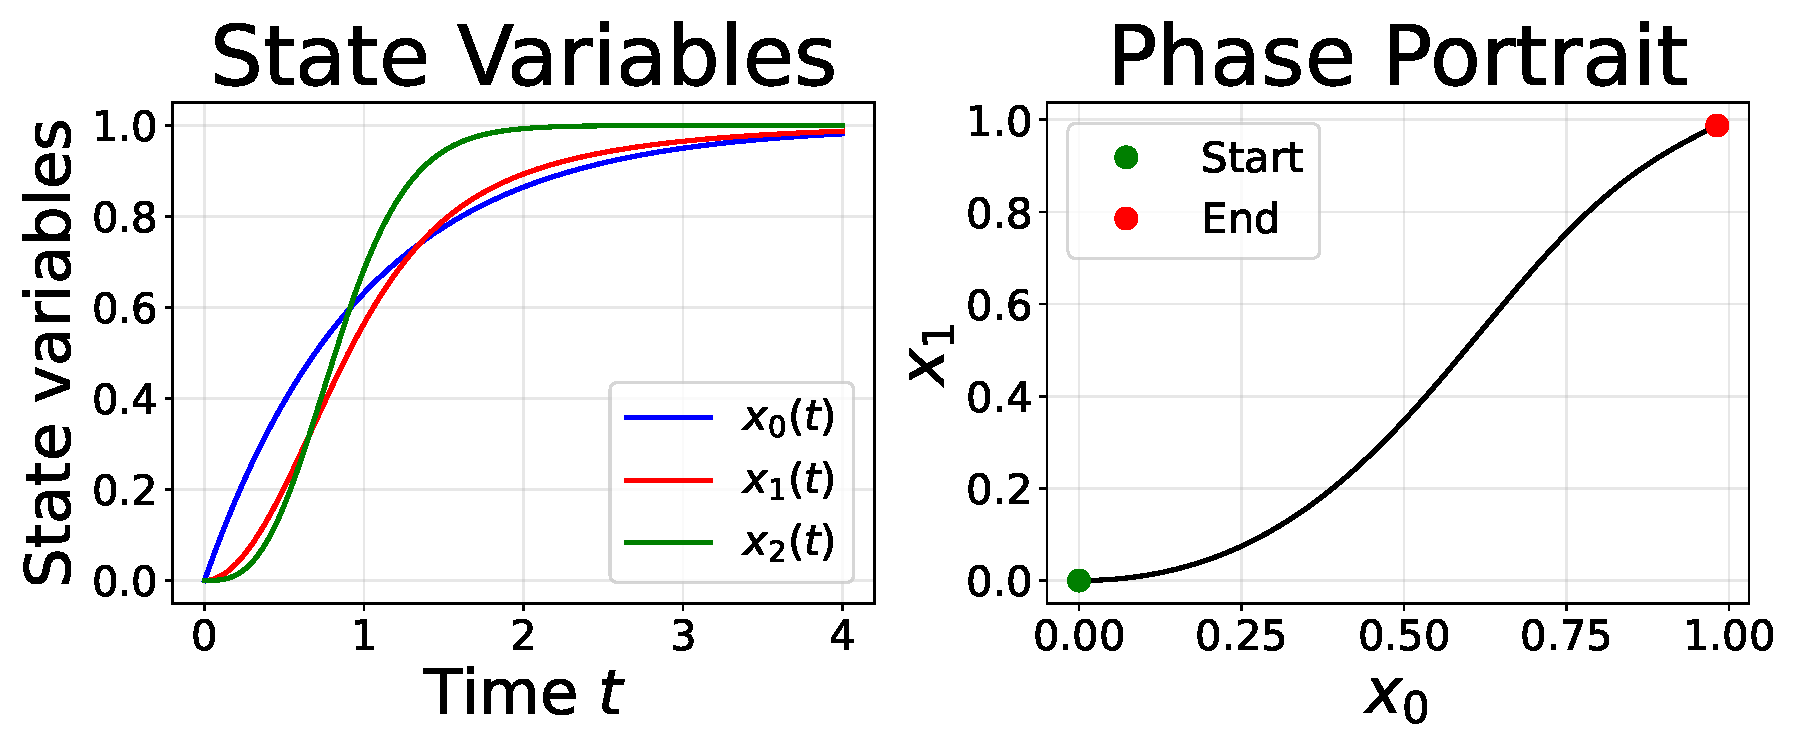
\includegraphics[scale=0.35]{../plots/dae_system.pdf}
\end{figure}
\end{frame}

\subsection{MICM Interface}

\section{MICM Backward Euler Solver}

\section{MICM Rosenbrock Solver}

\nocite{SanduI}
\nocite{SanduII}
\nocite{ODEsI}
\nocite{ODEsII}

\section{Bibliography}
\begin{frame}[allowframebreaks]{Bibliography}
\bibliographystyle{plainnat}
\bibliography{refs}
\end{frame}

\end{document}
